\newpage
\part{Platforma Gisquick}
\newpage

\section{Úvod do Gisquick}

Gisquick je webová mapová publikační platforma s otevřenými daty. Jejím účelem je snadné a rychlé publikování projektů vytvořených v programu QGIS, které je možné posléze prohlížet webovém rozhraní platformy Quisqick. 
Celá platforma se skládá z několika komponentů (jejich obecné fungování je popsáno v Části I, kapitole 1.2). Komponenty jsou následující.

\subsection{Komponenty}

\begin{itemize}
	\item\textit{Gisquick plugin} - jedná se o zásuvný modul pro program QGIS, pomocí kterého je možné existující projekt publikovat. Použití pluginu je prvním krokem k publikaci předem vytvořeného projektu. Při publikaci si může každý uživatel pomocí pluginu projekt nastavit tak, aby zobrazovaný předmět zájmu přesně odpovídal jeho požadavkům (možnost selekce jednotlivých vrstev, nastavení maximálního a minimálního měřítka, atd.). Gisquick plugin pracuje zcela odděleně od ostatních komponentů a jeho výstupem je složka obsahující všechny použité vrstvy, uložený projekt ve formátu .qgs a metadatový soubor obsahující dodatečné nastavení projektu.
	\item\textit{webový server} - webový server zpracovává dotazy ve formě OGC standardů, které posílá klient a následně odpovídá například ve formě mapových obrazů. Na straně webového serveru je použit framework Django, který je stejně jako Gisquick plugin psaný v jazyce Python.
	\item\textit{QGIS server} - jedná se o webový mapový server na základě kterého jsou vytvářeny mapové obrazy. Použití QGIS serveru je dáno skutečností, že veškeré mapové prvky zde vytvořené korespondují svým vzhledem s těmi vytvořenými v QGIS desktopové aplikaci. Díky tomu si může být uživatel jistý tím, že to co publikuje bude věrně odpovídat jeho původnímu projektu.
	\item\textit{webový a mobilní klient} - klient uživateli nabízí uživatelské rozhraní celé aplikace ve kterém se může orientovat a pomocí kterého interaguje s webovým serverem a tak mění zobrazovaný obsah. Právě této části spolu s Gisquick Pluginem byla je v této práci věnována největší pozornost.
\end{itemize}

\subsection{Uživatelské rozhraní}

\begin{figure}[h!]
	\centering
	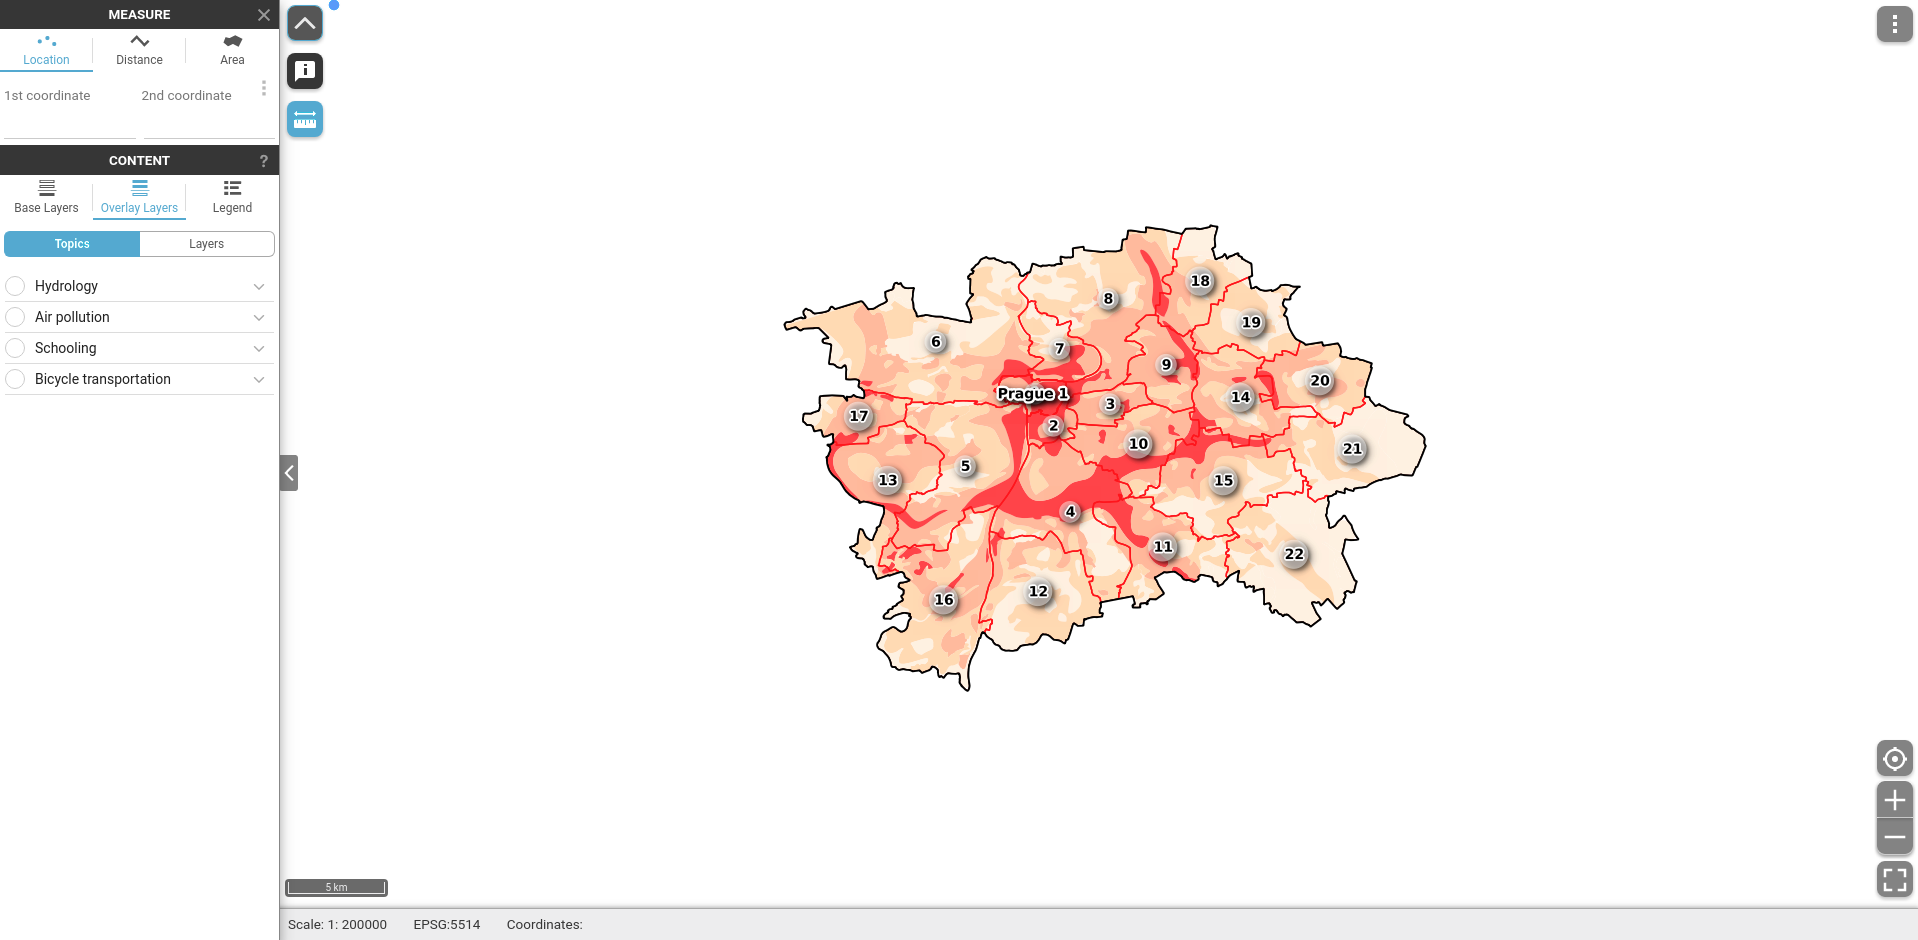
\includegraphics[width=0.9\textwidth]{../img/gisquick_ui.png}
	\caption{screenshot uživatelské rozhraní platformy Gisquick\cite{gisquick-prague}}
	\label{fig:gisquick-prague}
\end{figure}

Obrázek výše zachycuje webové uživatelské rozhraní Gisquick platformy. Jedná se o sadu velice jednoduchých a intuitivních nástrojů sloužících pro snadnou orientaci v publikovaném projektu, filtraci jednotlivých částí a provádění velice jednoduchých operací jako je například měření vzdáleností na mapě.

Uživatel má být schopný rychlé a intuitivní orientace v datech a samotné aplikaci. K tomu slouží postranní menu se správou vrstev spolu s menu nástrojů, které je v přiloženém obrázku rozbaleno. V postranním menu v horní části je právě aktivovaný nástroj sloužící k zjišťování souřadnic, měření vzdáleností a ploch. Hlavní část je věnována samotné interaktivní mapě. Ta poskytuje možnost změny velikosti a polohy zobrazovaného území.

\begin{figure}[h!]
	\centering
	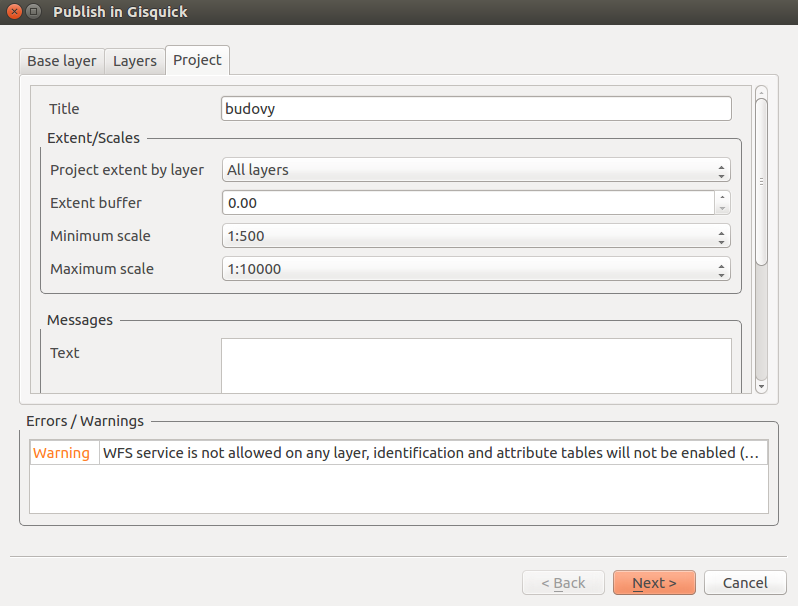
\includegraphics[width=0.7\textwidth]{../img/gisquick_plugin.png}
	\caption{screenshot uživatelské rozhraní Gisquick pluginu pro QGIS}
	\label{fig:gisquick-plugin}
\end{figure}

\newpage
Gisquick plugin rovněž disponuje uživatelským rozhraním, kde pomocí jednoduchého dialogového okna jsou nabízeny možnosti pro export vrstev. Jeho první část je rozdělena na tři záložky a stavovou řádku, kde se jsou vypisovány errory. V první záložce je možno nastavit podkladové vrstvy jako například Open Street Map, nebo Binq mapy. V další záložce je možno nastavit viditelnost jednotlivých vrstev. Při implementaci podpory pro časoprostorová data byly jednotlivé vrstvy rozšířeny o další nastavení. Tomu se bude práce věnovat detailněji v další části. V poslední záložce je obecné nastavení projektu. Další okno slouží k nastavení \textit{topics} nebo-li tématicky orientovaných vrstev \cite{gisquick-manual}. Předposlední stránka obsahuje pouze souhrn publikovaného projektu. A poslední zobrazuje výpis souborů, které se po zmáčknutí tlačítka \textit{Publish} vytvoří. Ty je poté nutné nahrát na Gisquick publikační server.

\newpage
\subsection{Použité technologie}
	
\begin{figure}[h!]
	\centering
	
\includegraphics[width=0.8\textwidth]{../img/technologies.JPG}
	\caption{loga níže popsaných softwarů}
	\label{fig:arcgis-time-settings}
\end{figure}	
	
\noindent
\textbf{Vue.js} - jedná se o moderní framework s otevřeným kódem napsaný v programovacím jazyce JavaScript jehož první verze byla vydaná začátkem roku 2014 Evanem You \cite{vue-history}. Jeho hlavní použití je vývoj uživatelského rozhraní aplikací, tedy na straně klienta. Uživatelské rozhraní je za pomoci Vue.js rozděleno na několik  komponent, kdy každá obsahuje vlastní javascriptové, html a css skripty. Jednotlivé komponenty dělají kód přehlednější a aplikace méně náročnější. Protože vždy jsou použity jenom ty komponenty, které koncový uživatel potřebuje. Mezi další výhody Vue.js patří mimo práce s komponenty jeho reaktivita, možnosti routingu a úpravu objektového modulu dokumentu (DOM).  

Původní verze webového klienta Gisquicku jsou psány za použití frameworku AngularJS. V současné chvíli je však celý klient vytvářen znovu za pomoci medernějšího Vue.js. Z toho důvodu bylo rozšíření platformy o podporu časoprostorových dat na straně klienta psáno ve stejném framevorku Vue.js. Pokud by se nástroj osvědčil pro jeho použití v produkční verzi, nebude nutné do budoucna kód přepisovat.

\newpage
\bigskip
\noindent
\textbf{PyQt} - PyQt je vazba pro programovací jazyk Python, která umožňuje využití frameworku pro Qt aplikace. Vazby jsou vytvořeny ve formě Python modulů a obsahují okolo jednoho tisíce tříd. Jedná se o kombinaci výhod nabízející jednoduchost Pythonu a obrovské schopnosti Qt dohromady. Díky tomu je možné jednoduše vytvářet grafické uživatelské rozhraní přímo za pomocí Pythonu. PyQt je software s otevřeným kódem, který byl vytvořen britskou firmou Riverbank Computing a je nabízen pod dvojí licencí GNU GPL v3 a komerční licencí společnosti Riverbank \cite{pyqt}.

\bigskip
\noindent
\textbf{Docker} - Docker je počítačový program s otevřeným kódem umožňující zapouzdření (izolaci) jednotlivých aplikací do kontejnerů. Vytvořený kontejner se nazývá \textit{Docker image}. Obecné pravidlo je použití pouze jedné aplikace pro jeden Docker kontejner. Docker image mohou být posléze spuštěny na jakémkoli hardwaru s operačním systémem Linux, nebo Windows, na který je Docker program nainstalovaný. Tato skutečnost má obrovskou výhodu pro nasazení aplikací do produkčních serverů, jejich sdílení s dalšími uživateli, nebo vytváření clusterů složených z mikroservis. Po spuštění aplikace v Docker kontejneru není vytvořen nový virtuální stroj, ale aplikace v kontejnerech využívají hostující operační systém. Výhod tohoto řešení spočívá v minimalizaci velikosti kontejneru.

Gisquick pro deploy svých komponent (mimo Gisquick pluginu) v produkční verzi využívá právě použití Docker kontejnerů. Tímto způsobem je možné celou Gisquick platformu jednoduše spustit na lokálních zařízeních. Vývoj je tak jednodušší, protože odpadá jakékoli nastavování vývojového prostředí. 

\bigskip
\noindent
\textbf{OpenLayers} - jedná se o knihovnu napsanou v programovacím jazyce JavaScript, která umožňuje správu a vizualizaci map ve webových prohlížečích. Jedná se o software s otevřeným kódem nabízející široké rozhraní pro tvorbu geografických aplikací. OpenLayers byly vytvořeny soukromou společností MetaCarta v roce 2005. Od roku 2007 spadají OpenLayers pod organizaci OSGeo.

\newpage
\section{Implementace nástroje pro Gisquick plugin}

%Následující kapitola popisuje způsob jakým byla platforma Gisquick respektive její komponenty rozšířeny o podporu práce s časoprostorovými daty. Jednotlivé podkapitoly zmiňují základní funkcionalitu, která byla nutná udělat a způsob její implementace.

V kapitole 3.1 jsou zmíněny výstupy z Gisquick pluginu. Jedná se o sloužku obsahující projekt ve formátu .qgs, data použita v projektu a metadatový textový soubor. Soubor obsahuje nastavení a popis dat použité na straně mapového serveru a webového klienta. Hlavním cílem úprav Gisquick pluginu bylo tedy vytvoření jednoduchého uživatelského rozhraní, které umožní definovat všechny potřebná data, pomocí kterých budou do metadatového souboru vepsány potřebné informace identifikující vrstvu jako časovou. Ty poté souží ve webovém klientu k inicializaci nástroje pro práci s časovými daty.

\subsection{Uživatelské rozhraní}

\begin{figure}[h!]
	\centering
	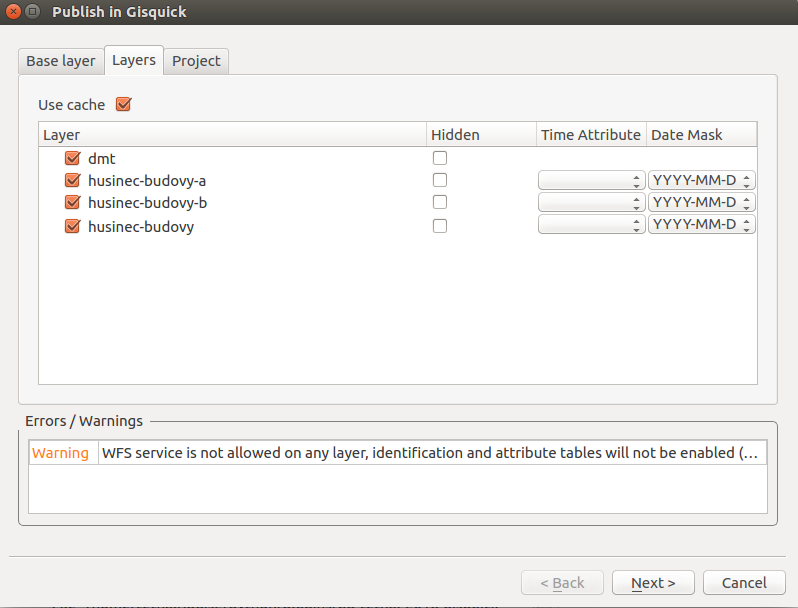
\includegraphics[width=0.9\textwidth]{../img/gisquick-plugin.png}
	\caption{nastavení vrstev v Gisquick pluginu}
	\label{fig:arcgis-time-settings}
\end{figure}

Obrázek 11 zobrazuje dialogové okno publikace projektu pomocí Gisquick pluginu. V prvním kroku publikace v záložce vrstvy \textit{Layers} je přidáno nové nastavení pro vektorové vrstvy. V Případě rastrových, jako je například v obrázku zvolená vrstva dmt, možnost nastavení časových vrstev není možná.

Ve sloupci \textit{Time Attribute} jsou v roletovém menu vypsány všechny atributy každé vrstvy. Implicitní nastavená hodnota je prázdný textový řetězec. Zde je nutné pro každou časovou vrstvu vybrat atribut, který obsahuje časové hodnoty. 

Sloupec \textit{Date Mask} obsahuje roletové menu s datovými masky, které určují jakým způsobem budou časová data na webovém klientu zobrazena. Díky tomuto nastavení je, nehledě na formát časového atributu, možné publikovat v časovém formátu, na který jsou cíloví uživatele zvyklí. V případě volby formátu je nutné znát původní data. Přejde se tím situacím kdy uživatel zvolí formát zobrazení dat pouze roky, zatímco původní data jsou v rozpětí jednoho dne.

Jestli jsou časové vrstvy dobře nastaveny se lze v předposledním kroku publikace přesvědčit v souhrnu publikovaného projektu.
%obrazek ze souhrnu (az bude)

\subsection{Funkcionalita}

Poté co uživatel v záložce Vrstvy nastaví všechny požadované parametry může svou volbu potvrdit tlačítkem \textit{Next}, které spustí výpočet a zobrazí další krok publikace.

Do výpočetního procesu se dostanou pouze ty vrstvy, které splňují dvě podmínky. Jejich časový atribut \textit{Time Attribute} musí existovat. Tato podmínka eliminuje výpočet nad rastrovými vrstvy. Dále je nutné, aby byl nastavený časový atribut jiný než prázdný textový řetězec. Tímto způsobem se do výpočtu dostanou pouze ty vrstvy, které uživatel výběrem atributu označí jako časové.

Výpočet probíhá pro jednotlivé vrstvy splňující vstupní podmínky totožně. Pro každou mapovou vrstvu je volána metoda \verb|get_time_info|.

V prvním kroku je metodou \verb|validate_time_attribute| vytvořena validační maska. Jedná se o pole, které svou velikostí odpovídá počtu mapových prvků \textit{Features} ve vrstvě. Každý prvek validační masky může nabývat dvou hodnot. Buďto obsahuje formát časového textového řetězce \textit{time string}, ve kterém je časová hodnota uložena. Pokud však časová hodnota není v textovém řetězci, nebo její časový formát textového řetězce neodpovídá podporovaným formátům, je do daného prvku validační masky uložena hodnota \textit{-1}. Podporované formáty jsou explicitně vypsány ve zdrojovém kódu Gisquick pluginu v proměnné \verb|datetime_mask_array|.

Pro vrstvu obsahující šest prvků, kdy pouze pět z nich má validní datum a to ještě v odlišných časových formátech může validační maska vypadat následovně:

\begin{verbatim}
[
  '%Y-%m-%d',
  '%Y-%m-%d',
  -1,
  '%Y-%m-%dT%H:%M:%S',
  '%Y-%m-%dT%H:%M:%S',
  '%Y-%m-%dT%H:%M:%S'
]
\end{verbatim}

Během vytváření validační masky jsou rovnou data kontrolována metodou \verb|validate|. Díky tomu je možné zjistit jak maska vypadá aniž by bylo nutné její jednotlivé prvky procházet. Po její vytvoření jsou pouze tři možné scénáře jsou možné.

%specialni znak

\begin{itemize}
	\item\textit{Data nejsou validní} - znamená, že ani jeden hodnota v zadaném časovém atributu nemá validní časovou hodnotu. Validační maska tedy obsahuje pouze hodnoty \textit{-1}. Výpočet je v tomto případě ukončen.
	\item\textit{Data jsou validní a obsahují pouze jeden časový formát} - v tomto případě je zjištěno, jestli je časový formát neobsahuje speciální znak, který by jeho použití pro následnou filtraci mapových prvků v původní podobě znemožnil použít.
	\begin{itemize}
		\item\textit{Obsahuje speciální znak} - v tom případě se pokračuje způsobem stejným jako v případě \textit{Data jsou validní, ale obsahují více časových formátů} popsaném níže.
		\item\textit{Neobsahuje speciální znak} - časové textové řetězce jsou metodou \\* \verb|get_min_max_mask| za pomocí formátu, zjištěného časového z validační masky, převedeny do časového formátu \textit{UNIX TIME}. Z těchto hodnot jsou poté zjištěny jejich maximální a minimální hodnota.
		Pro získání časového formátu z validační masky je použita metoda \verb|most_common|, která vybere nejvíce zastoupený prvek v poli. K její funkčnosti je tedy nutné nejprve metodou \verb|remove_values_from_list| odstranit záznamy obsahující hodnoty \textit{-1}.
	\end{itemize}
	\item\textit{Data jsou validní, ale obsahují více časových formátů} - jedná se tedy o validní nekonzistentní data. Pro tento případ slouží metoda \\* \verb|create_unix_time_attribute|, která má návratovou hodnotu stejnou jako metoda \verb|get_min_max_mask|. K tomu aby vrstvu s časovými hodnoty bylo možné označit za časovou je v této metodě je nutné metodou \\* \verb|create_new_attribute| vytvořit nový atribut, který obsahuje časové hodnoty v jednotném formátu. Toho je docíleno pomoci validační masky, kdy se prochází jednotlivé hodnoty. Pokud pro záznam existuje formát časového textového řetězce, je jeho hodnota převedena do formátu \textit{UNIX TIME}. Ten je následně uložen v novém atributovém sloupci metodou \verb|changeAttributeValues|. V případě nevalidní časové hodnoty je pole prázdné. Na základě hodnot v atributu obsahující časové hodnoty ve formátu \textit{UNIX TIME} je určena hodnota minimálního a maximálního časového atributu.
	V případě, že nový atribut již jednou vytvořen byl, jsou jeho hodnoty přepsány.
\end{itemize}

\begin{figure}[h!]
	\centering
	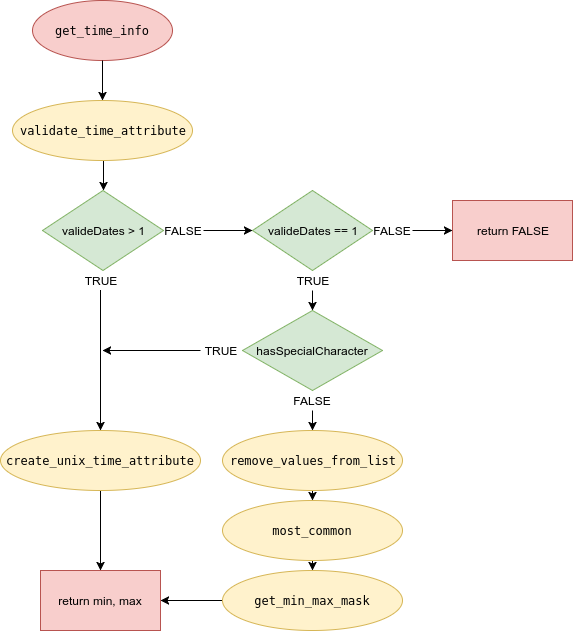
\includegraphics[width=0.8\textwidth]{../img/getTimeInfo.png}
	\caption{vývojový diagram publikace časové vrstvy}
	\label{fig:plugin-chart}
\end{figure}

Posledním krokem je poté pouze export zjištěných hodnot do metadatového souboru. Pro každou časovou vrstvu je vypsána časový formát pro zobrazení hodnot na webovém klientu. Dále název časového atributu, minimální a maximální hodnota časového atributu ve formátu \textit{UNIX TIME} a další parametry které budou popsány a vysvětleny dále. V případě, že data jsou validní a není vytvořen nový atribut obsahující časové hodnoty ve formátu \textit{UNIX TIME} je vypsán formát obsažený ve validační masce. Pokud je pomocný atribut použit, je vypsán jeho název.

%vyvojovy diagram

\subsection{Metadatový soubor}

Metadatový soubor (viz. kapitola 3.1 \textit{Gisquick plugin}) je textový soubor, který vniká publikací projektu pluginem Gisquick. Obsahuje množství informací, které jsou nutné pro správnou konfiguraci straně mapového serveru a webového klienta. V případě časových vrstev jsou dodatečné informace použité pouze na straně webového klienta. 

Pokud jsou vrstvy při publikaci označeny jako časové a jejich data jdou validní, jsou do nich vepsány následující hodnoty:

\begin{itemize}
	\item\textit{unix} - parametr unix nabývá hodnoty \textit{TRUE} v případě, že byl vytvořen nový atribut s časovými hodnoty ve formátu \textit{UNIX TIME}. Slouží webovému klientu k určení zdali k filtrování časové vrstvy má použít daný formát, nebo \textit{UNIX TIME}.
	\item\textit{originalTimeAttribute} - zde je uložen název časového atributu. Parametr slouží k určení atributu při filtrování časové vrstvy. 
	\item\textit{outputDatetimeMask} - obsahuje formát časového řetězce, který si uživatel zvolil v roletovém menu \textit{Date Mask}. Použití tohoto parametru je pouze pro možnost definice formátu zobrazení data a času v časovém nástroji.
	\item\textit{timeValues} - jedná se o pole obsahující minimální a maximální hodnotu časového atributu ve formátu \textit{UNIX TIME}. Dle těchto hodnot je inicializovaný časový posuvník. 
	\item\textit{inputDatetimeMask} - tento parametr je vytvořen pouze pokud není nutné vytvářet nový atribut obsahující hodnoty ve formátu \textit{UNIX TIME}. Parametr obsahuje formát časového řetězce pro zvoleného časového atributu. Díky tomuto parametru může být pro potřeby filtrování časové vrstvy převedena hodnota učená na časovému posuvníku do stejného časového formátu v jakém je uložena. 
	\item\textit{timeAttribute} - parametr je vytvořen pouze pokud je nutné vytvářet nový atribut obsahující hodnoty ve formátu \textit{UNIX TIME}. Obsahuje název nově vytvořeného atributu. Parametr slouží stejně jako \textit{originalTimeAttribute} k určení atributu při filtrování časové vrstvy.  
\end{itemize}

\newpage
\bigskip
\noindent

Níže je ukázka části metadatového souboru. Ta obsahuje dvě vrstvy, kdy každá z nich má odlišné parametry. Pro kompaktnost ukázky zde parametry, které se netýkají implementovaného rozšíření zobrazeny nejsou: 

\begin{verbatim}
{
	"unix": false, 
	"timeValues": [
	1309471200.0, 
	1507672800.0
	], 
	"input_datetime_mask": "YYYY-MM-DD", 
	"output_datetime_mask": "YYYY-MM-DD", 
	"original_time_attribute": "platiod", 
}, 
{
	"timeAttribute": "UTconvert", 
	"unix": true, 
	"timeValues": [
	1309471200, 
	1507672800
	], 
	"output_datetime_mask": "HH:mm", 
	"original_time_attribute": "platiod1", 
}
\end{verbatim}

\newpage
\section{Implementace nástroje do webového klienta}
Webový klient obsahuje hlavní část implementace rozšíření pro podporu časoprostorových dat. Jedná se o intuitivní nástroj, který umožňuje filtrovat obsah jednotlivých vrstev na základě jejich časového parametru. Časový interval je možné nastavit pomoci posuvníku, nebo přímo změnit ručně. Nástroj na webovém klientu umožňuje dále vytvářet jednoduché animace. Uživatel má rovněž možnost zmíněnou filtraci mapových prvků provádět pro jednotlivé vrstvy, nebo na více vrstev současně. 

\subsection{Uživatelské rozhraní}

\begin{figure}[h!]
	\centering
	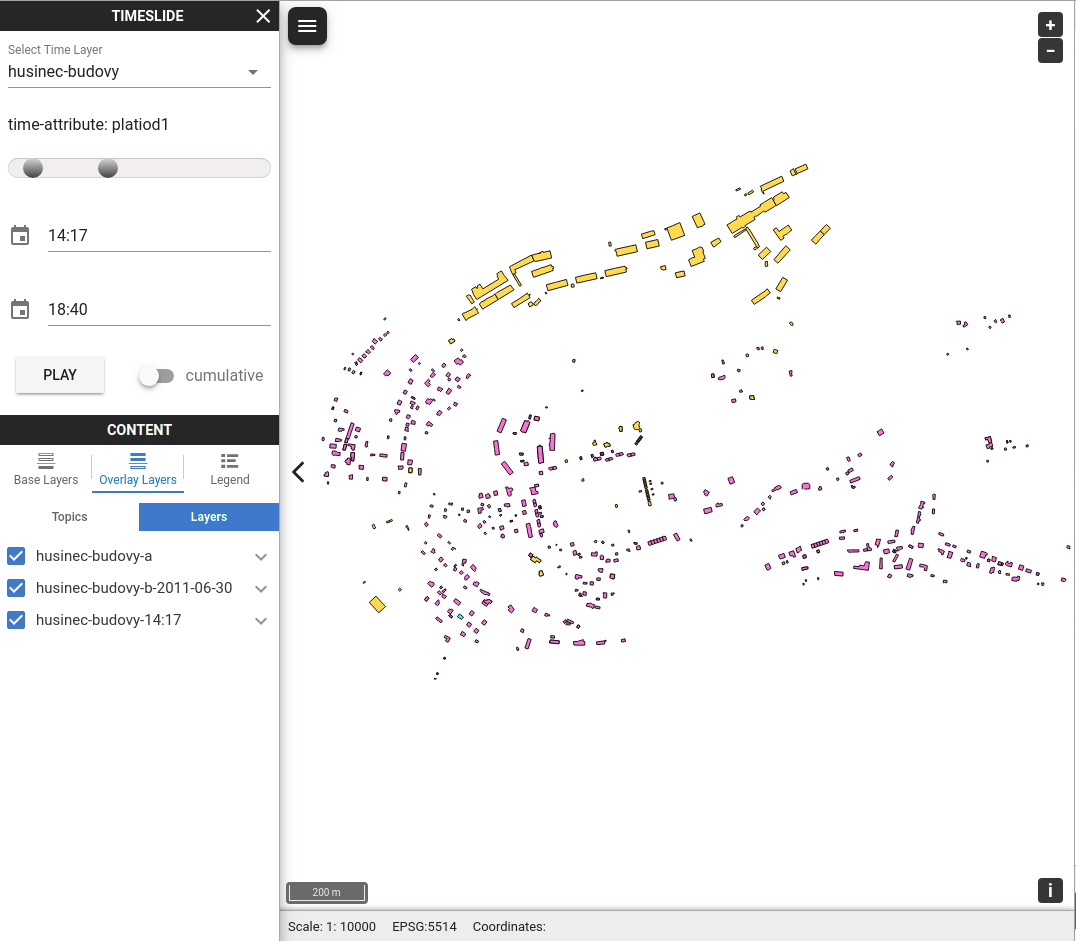
\includegraphics[width=1\textwidth]{../img/gisquick-time-tool.png}
	\caption{webové rozhraní Gisquick platformy s aktivovaným nástrojem pro páci s časoprostorovými daty}
	\label{fig:arcgis-time-settings}
\end{figure}

Celý nástroj je ukrytý v postranním menu a obsahuje jen několik prvků, které však uživateli poskytují velké množství operací. Všechny jsou zobrazeny v obrázku 12 a jednotlivě se jedná o:

\begin{itemize}
	\item\textit{roletové menu s výběrem časové vrstvy} - v případě aktivace nástroje je toto pole jediný prvek, který je uživateli zobrazen. Jako první krok je totiž nutné vybrat časovou vrstvu, jejíž mapové prvky budou filtrovány. Toho lze docílit pomocí zmíněného roletového menu, které obsahuje všechny vrstvy, které byly při jejich exportu označeny jako časové. Dále je zde možnost "All visible layers", která uživateli umožní filtraci více vrstev zároveň.
	\item\textit{jméno časového atributu} - tento prvek neumožňuje uživateli jakoukoli interakci a má tedy čistě informativní charakter. Je zde vypsán atribut vrstvy, ve kterém jsou časové hodnoty použité při filtraci uloženy. Jeho existence je přínosná především v případě kdy projekt obsahuje více časových vrstev s odlišným časovým parametrem. V případě filtrace více vrstev najednou je možné filtrovat pouze vrstvy se stejným parametrem. Uživatel je tedy tomto případě informován pro jaký parametr jsou vrstvy filtrovány.
	\item\textit{dvojitý časový posuvník} - jedná se posuvník se dvěma šoupátky. Díky němu je možné snadno a rychle data filtrovat. Uživatel tak ihned získá představu o jejich časové ose. Minimum a maximum posuvníku odpovídá minimu a maximu intervalu časových hodnot jednotlivé vrstvy. Pro více vrstev se jedná o sjednocení intervalů. Krok je vždy určen jako jedna setina intervalu hodnot posuvníku. Je tedy zřejmé, že posuvník slouží především pro rychlou filtraci než přesnou definici hledaného intervalu. 
	\item\textit{časové štítky} - na dvou řádcích jsou dvě pole s minimálním a maximálním datem filtrovaných časových hodnot. Tato pole slouží k přesné definici časového úseku. K tomu slouží integrovaný kalendář s hodiny. Časový formát zobrazený v těchto polích je nutné definovat při publikaci projektu. Pokud formát neobsahuje možnost zobrazení minut, nebo hodin v tom případě se možnost zadání hodin a minut nenabízí. Stejným způsobem není nabídnut možnost filtrování za pomoci kalendáře v případě, že časový formát obsahuje jen hodiny, nebo minuty.
	\item\textit{animační tlačítko} - tlačítkem \textit{PLAY} je možné spustit animování aktivní časové vrstvy. Po jeho aktivaci je vždy po jedné sekundě zvyšována hodnota horní hranice intervalu časových hodnot a to o jeden krok posuvníku. Pokud je animace aktivovaná změní se tlačítko na \textit{STOP}. Tím je tak možné animování zastavit.
\end{itemize}

\subsection{Princip časové filtrace}
Jak bylo zmíněno v kapitole 2.6, QGIS server nepodporuje v operaci \textit{GetMap} parametr \textit{TIME}. Z toho důvodu je nutné použít obdobnou metodu, kterou používá MapServer, a to nahrazení parametru \textit{TIME} parametrem \textit{FILTER}.

\noindent
Parametr \textit{FILTER} lze použít v operaci \textit{GetMap} následovně \cite{qgis-service}:
\begin{verbatim}
http://myserver.com/?
REQUEST=GetMap
&LAYERS=mylayer1,mylayer2
&FILTER=mylayer1:"OBJECTID" = 3;mylayer2:'text' = 'something'&....
\end{verbatim}

Tato skutečnost dovoluje filtrovat časové vrstvy na základě jejich atributu obsahujícího časové hodnoty a samotné hodnoty časového atributu. Lze tak filtrovat jednu i více vrstev najednou. Za použití speciálních znaků jako jsou \textit{‘AND’, ’OR’, ’IN’, ’=’, ’<’, ’>=’,  ‘>’, ’>=’, ’!=*,’(‘,’)’} lze rovněž filtrovat intervaly hodnot i jejich sjednocení.

V implementovaném nástroji pro časovou filtraci je při filtrování použit dvojitý časový posuvník. Proto je obsah parametru \textit{FILTER} vždy tvořen jako textový řetězec, který v obecné formě vypadá následovně:

\begin{verbatim}
mylayer1:
"timeAttribute" >= 'lowerValue' 
AND 
"timeAttribute" <= 'upperValue'
\end{verbatim}

Parametr \textit{FILTER} podporuje zadané hodnoty ve datovém typu textového řetězce, nebo jako celé číslo. Pro zachování konzistence výsledků filtrování je nutné, aby datový typ a časový formát hodnoty vstupující do parametru \textit{FILTER} korespondovaly příslušným časovým atributem. Z toho důvodu je při publikaci projektu ve speciálních případech nutné vytvoření nového atributu. Ten obsahuje hodnoty časového atributu převedeny do formátu \textit{UNIX TIME}. To dovoluje k časovým hodnotám přistupovat jako k celočíselným hodnotám. V případě časového filtrování této vrstvy není tedy použit námi zvolený časový atribut, ale nově vytvořený. Nutnost vytvářet nový atribut je v následujících případech:

\begin{itemize}
	\item\textit{časový atribut obsahuje validní ale nekonzistentní časové řetězce} - v procesu publikace je provedena validace hodnot časového atributu. Pokud je zjištěno, že atribut obsahuje validní záznamy ve více časových formátech nebylo by v takovém případě možné oba tyto formáty použít. Proto je pro konkrétní vrstvu nutné vytvořit nový atribut s jednotným formátem (v tomto případě \textit{UNIX TIME}). Tato zkutečnost je poté zanesena do metadatového souboru.
	\item\textit{časový atribut obsahuje jeden validní formát se speciálními znaky} - při filtraci mapových prvků na základě časového řetězce nelze použít všechny běžně používané formáty. Například při použití data v textovém formátu 'YYYY-MM-DDTHH:mm:SS', kdy je použit znak 'T' oddělující datum a čas, nelze textový řetězec v parametru \textit{FILTER} použít.
\end{itemize}

\subsection{Inicializace nástroje}

Pokud není volba \textit{Use cache} při publikování projektu vypnutá (viz. obrázek 11),  používá Gisquick webový klient pro zobrazování mapových vrstev předem vytvořených mapových dlaždic uložených v mezipaměti serveru. Pro možnosti filtrace vrstev na základě jejich časové hodnoty parametru však tento způsob nelze aplikovat. Bylo by totiž nutné vytvořit mapové dlaždice pro všechny možné časové intervaly a kombinace vrstev. Z toho důvodu je při aktivaci nástroje pro práci s časoprostorovými daty použit \textit{Lifecycle Hook Created}. Jedná se o funkci, která se spustí jakmile je Vue komponent inicializován. V ní je původní instance třídy \textit{ImageLayer} uložena do proměnné \textit{originalLayer} a skryta. Následně je vytvořena instance nová, která obsahuje stejné vrstvy jako původní. Ta je poté nastavena jako aktivní. Pokud je nástroj vypnut je použita původní instance a mapa je tedy opět v původním nastavení.

\subsection{Filtrace jedné časové vrstvy}

První a také jediný krok, který lze po inicializaci časového nástroje udělat je volba časové vrstvy. Zde je možno zvolit jednotlivé časové vrstvy (viz, kapitola 4.1), nebo filtraci všech viditelných časových vrstev. Pokud je vybrána možnost filtrace mapových prvků pouze jedné vrstvy, je tato vrstva v případě jejího skrytí znovu zviditelněna. Následný postup je popsán dále. 

\bigskip
\noindent \textbf{Inicializace}

Nejprve nutná inicializace časového posuvníku, na něm jsou závislé další uživatelské prvky jako například \textit{časové štítky}. Jeho minimální a maximální hodnota je získána z metadatového parametru \textit{timeAttribute} (viz. kapitola 4.3). Velikost kroku posuvníku určena jako setina rozdílu jeho maximální a minimální hodnoty. Metoda \verb|setSliderValue| inicializuje hodnoty šoupátek na jejich poslední použité. V případě, že nebyla vrstva ještě filtrována, je hodnota levého šoupátka rovna minimu časového posuvníku a hodnota pravého šoupátka o krok časového posuvníku větší. 

Stejně jako hodnoty parametru \textit{timeAttribute}, tak hodnoty šoupátek jsou v časovém formátu \textit{UNIX Time}, tedy jako datový typ \textit{Integer}. \textit{Vue.js} umožňuje nastavení \textit{Watched Property}. Takto jsou nastavené proměnné hodnoty šoupátek. Pokud se tedy jedna z hodnot změní je spuštěna metoda, která provede převod původního celočíselného časového formátu \textit{UNIX Time} do časového formátu \textit{OutputDatetimeMask} zvoleného během publikace projektu (viz. kapitola 4.1, 4.3). Jakmile je tedy časový posuvník inicializován, jsou ihned inicializovány i časové štítky časovou hodnotou v daném formátu.

\bigskip
\noindent \textbf{Filtrace}

%to je spis dokumentace
%Změnu obsahu mapy na základě filtrace jejích prvků lze provést dvojím způsobem. Buďto změnou polohy šoupátek časového posuvníku, v tom případě se mapový obsah aktualizuje až po uvolnění šoupátka. Druhý způsob je výběr přesného data a času v časových štítcích. Mapa se tak aktualizuje pouze když je výběr potvrzen tlačítkem \textit{"OK"}. To dovoluje uživateli změnit své rozhodnutí během samotné filtrace. 

Způsob, jakým je aktualizována mapa na základě změny časových hodnot je popsána v dokumentaci časového nástroje. Zde je popsán princip, kterým je mapový obraz aktualizován.

Při spuštění časové filtrace je v metodě \verb|updateSingleLayer| provedeno několik po sobě jdoucích operací:
\begin{itemize}
	\item\textit{detekce předem filtrovaných vrstev} - nejprve je nutné zjistit, zda-li ostatní viditelné vrstvy již filtrovány byly. V takovém případě je nutné do parametru \textit{FILTER} zahrnout nastavení předem filtrované vrstvy. Pokud by tak nebylo provedeno, z předem filtrovaných vrstev by byly zobrazeny všechny jejich prvky. To je provedeno metodou \verb|getFilterFromLayers|, která vrací textový řetězec obsahující obsah parametru \textit{FILTER}  (viz. kapitola 5.2) časových vrstev, které byly již předem filtrovány.
	\item\textit{sestavení filtru pro danou vrstvu} - další krok zahrnuje vytvoření obsahu parametru \textit{FILTER} pro právě filtrovanou vrstvu. Tento krok se liší v závislosti na existenci pomocného atributu s hodnoty ve formátu \textit{UNIX TIME} (viz. kapitola 4.2). Parametr \textit{unix} v metadatovém souboru (kapitola 4.3) obsahuje informaci o jeho vytvoření.
	\begin{itemize}
		\item\textit{unix = TRUE} - znamená to, že filtrace není provedena nad hodnoty časového atributu, ale pomocného atributu. Pro tuto kofiguraci je textový řetězec sestaven pouze z parametrů poskytovaných metadatovým souborem. Pro časovou hodnotu je přímo použita hodnota posuvníku, která je v časovém formátu \textit{UNIX TIME}.
		\item\textit{unix = FALSE} - v tomto případě je nutné nejprve časové hodnoty převést z formátu \textit{UNIX TIME} do textového řetězce, který svým časovým formátem odpovídá formátu časového atributu pro danou vrstvu. Formát pro záznamy časového atributu je součástí metadatového souboru jako \textit{inputDatetimeMask} (viz. kapitola 4.3). Sestavení textového řetězce je poté obdobné jako v předchozím případě.
	\end{itemize}
	Na konci tohoto kroku jsou poté spojeny dohromady obsahy parametru \textit{FILTER} z ostatních časových vrstev a nově vytvořený.
	%$overlays object
	\item\textit{nastavení filtrované vrstvy} - tento krok ne nezbytný z několika důvodů. Je nutné uložit hodnoty časového posuvníku v případě že vrstva bude v budoucnu filtrována znovu. Dále je nutné uložit použitý obsah parametru \textit{FILTER}, který je použit při filtrování ostatních časových vrstev. Jako poslední věc je změněn název vrstvy tak, aby obsahoval její jméno spolu s časovou hodnotou. Tímto způsobem uživatel ihned ví, které vrstvy byly již filtrovány.
	\item\textit{provedení operace GetMap} - v posledním kroku je metodou \verb|updateParams| poslán požadavek na server obsahující parametr \textit{FILTER} s obsahem složeným z filtru pro všechny viditelné časové vrstvy. Server vrátí v odpovědi mapový obraz s filtrovanými mapovými prvky, pomocí kterých je původní obsah mapy nahrazen.
\end{itemize}

\begin{figure}[h!]
	\centering
	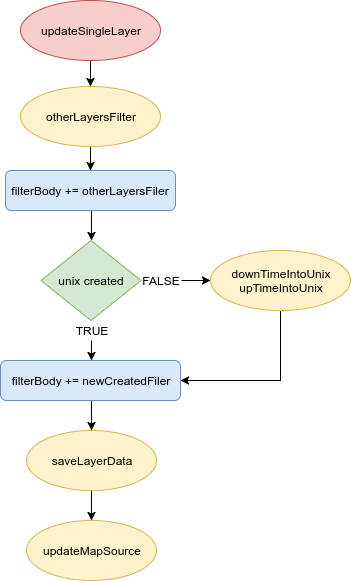
\includegraphics[width=0.5\textwidth]{../img/getSingleLayer.png}
	\caption{vývojový diagram filtrace více časových vrstev najednou}
	\label{fig:single-chart}
\end{figure}

\subsection{Filtrace všech viditelných časových vrstev}

Možnost selekce více vrstev je možné aktivovat v roletovém menu obsahujícím jednotlivé časové vrstvy. Možnost \textit{Select all visible layers} umožní provádět filtraci mapových prvků pro všechny viditelné časové vrstvy najednou.

\bigskip
\noindent \textbf{Inicializace}

Jednotlivé časové vrstvy mohou obsahovat navzájem odlišné časové atributy, které v jistých případech nedovolují společnou filtraci. Například pokud by projekt obsahoval dvě odlišné časové vrstvy, kdy jedna by zachycovala časový průběh v intervalu jednoho dne a druhá v intervalu jednoho roku. Výsledný krok časové filtrace by v takovém případě nebyl schopný postihnout nekonzistentní rozdělení dat vůči společné časové ose. Z toho důvodu je při výběru možnosti \textit{Select all visible layers} nejprve zjištěno, zdali viditelné časové vrstvy mají zvolen stejný, nebo odlišný časový atribut. Tato zkutečnost je zjištěna metodou \verb|checkMultipleAttributes|, která pro všechny viditelné časové vrstvy zjistí unikátní časové atributy a uloží je do pole. Pokud takové pole obsahuje více, než jeden prvek je zobrazeno další roletové menu ve kterém je nutné časový atribut specifikovat.

Při inicializaci časového posuvníku je nutné brát v potaz odlišné časové intervaly pro jednotlivé vrstvy. Metoda \verb|getSliderRange| postupně projde viditelné časové vrstvy a z hodnot jejich \textit{timeValues} (viz kapitola 4.3) určí celkové maximální a minimální hodnoty. Tímto způsobem je zajištěno, že všechny hodnoty časového atributu pro všechny časové vrstvy budou náležet intervalu časového posuvníku. Hodnoty šoupátek jsou nastaveny na minimální hodnoty intervalu časového posuvníku, resp. na hodnotu, která je o časový krok větší. Není přitom zohledňováno předchozí použití časových vrstev při jejich filtraci.

Dále je nutné zajistit, aby časové hodnoty zobrazované ve webovém klientu, při filtraci více vrstev najednou, měly společný časový formát. časový formát je pro jednotlivé vrstvy definovaný v metadatovém souboru (viz kapitola 4.3). Metoda \verb|setDateMask| má za úkol mezi časovými formáty filtrovaných vrstev najít takový, který poskytuje nejdetailnější zobrazení. Pokud tedy jedna z vrstev má nastaveno zobrazování minut, je její časový formát upřednostněn. Metoda pro jednotlivé časové formáty nejprve zjišťuje zda-li obsahují zároveň roky, hodiny a minuty. Pokud ano je první nalezený formát použit. Pokud tomu tak není je hledán formát obsahující alespoň roky. V případě, že ani takový není nalezen, je použit časový formát první časové vrstvy.

Pro správné zobrazení kalendáře a hodinového ciferníků pro výběr hodnot časových štítků je nutné zjistit, zdali vybraný časový formát obsahuje datum a čas. K tomu slouží metoda \verb|maskIncludeDate|. Na základě jejího výsledku je skryta možnost výběru časových hodnot pomocí kalendáře. Zobrazení hodinového ciferníku je řešeno obdobně s tím rozdílem, že k detekci času v časovém formátu je použito JavaScriptové metody \verb|includes|.

\bigskip
\noindent \textbf{Filtrace}

Princip a jednotlivé kroky samotné filtrace mapových prvků pro všechny zobrazené časové vrstvy odpovídají popsanému principu pro filtraci jednotlivých vrstev. Je zde však jedna podstatná změna při vytváření obsahu parametru \textit{FILTER}. V metodě \verb|updateMultipleLayers| je oproti metodě \verb|updateSingleLayer| cyklus, který prochází jednotlivě všechny viditelné časové vrstvy a zjišťuje jestli jejich časový atribut je shodný s časovým atributem všech zobrazovaných viditelných časových vrstev. Dále je z jednotlivých vrstev sestaven obsah parametru \textit{FILTER}. Pro každou vrstvu mohou nastat dva případy:
	\begin{itemize}
		\item\textit{atribut není totožný} - pokud již byla vrstva předem filtrována obsahuje předem použitý obsah parametru \textit{FILTER}. Ten je v tomto případě zjištěn a přidán do nově vytvářeného obsahu.
		\item\textit{atribut je totožný} - časová vrstva je filtrována a je tedy nutné sestavit obsah parametru znovu. Tento princip je stejný jako v případě filtrace jednotlivé vrstvy. Obsah parametru je rovněž přidán do nově vytvářeného obsahu. Pro vrstvu jsou navíc uloženy stejné hodnoty jako v případě filtrace jednotlivých vrstev. Pokud by tedy vrstva byla filtrována samostatně inicializuje se časový posuvník naposledy uloženými hodnoty. 
	\end{itemize}
Pokud jsou všechny viditelné časové vrstvy zpracovány je nově vytvořený obsah parametru \textit{FILTER} použit při operaci \textit{GetMap} stejným způsoben jako u filtrace jednotlivé vrstvy.

\begin{figure}[h!]
	\centering
	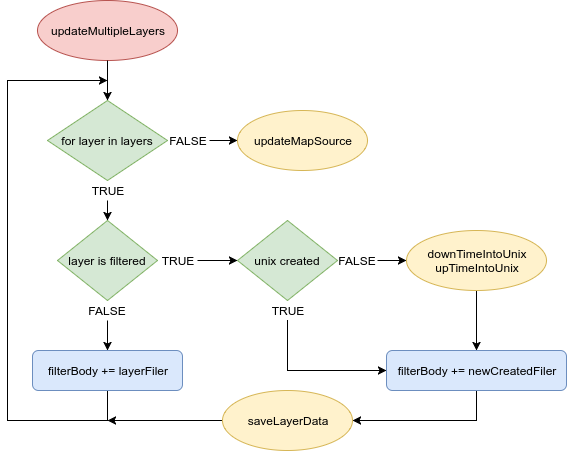
\includegraphics[width=0.9\textwidth]{../img/getMultipleLayers.png}
	\caption{vývojový diagram filtrace více časových vrstev najednou}
	\label{fig:multiple-chart}
\end{figure}

\subsection{Animace filtrace}

Jak při možnosti filtrace jednotlivé vrstvy, tak při více vrstev najednou je možnost provádět filtraci mapových prvků automatizovaně a vytvářet tak jednoduché animace. K tomu slouží tlačítko \textit{PLAY} na spodní straně nástroje viz. kapitola 5.1.

Jedná se jednoduchou metodu \verb|animate|, která v daném intervalu mění hodnotu časového posuvníku. Tato metoda pouze kontroluje hodnotu proměnné \textit{animateStop}. Pokud je tato hodnota FALSE, je volána metoda \verb|newFrame|. Tato metoda při každém svém zavolání zkontroluje hodnotu checkoboxu cumulative:
\begin{itemize}
	\item\textit{cumulative = TRUE} - pokud je hodnota horního šoupátka menší než naximální hodnota časového posuvníku, je zvýšena o krok posuvníku. Pokud je vyšší, je zvýšena hodnota dolního šoupátka.
	\item\textit{cumulative = FALSE} - pokud je hodnota horního šoupátka menší než naximální hodnota časového posuvníku, jsou zvýšeny obě hodnoty šoupátek o krok časového posuvníku.
\end{itemize}
Po zvýšení hodnot zavolá metodu \verb|getNewUrl| (viz. kapitola 5.4), která aktualizuje mapový obsah podle nově nastavených filtrovaných hodnot. Nakonec v případě, že hodnota \textit{animateStop = FALSE}, zavolá rekurzivně sama sebe s časovou prodlevou jedna sekunda. 

\begin{figure}[h!]
	\centering
	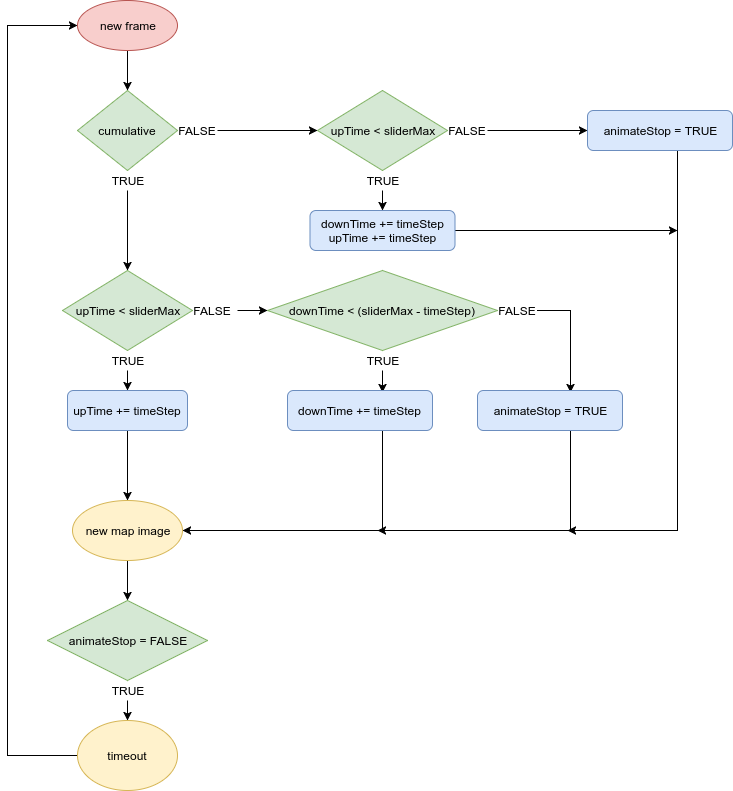
\includegraphics[width=0.9\textwidth]{../img/animate.png}
	\caption{vývojový diagram metody animate}
	\label{fig:animate-chart}
\end{figure}